\documentclass{article}


\usepackage{arxiv}

\usepackage[utf8]{inputenc} % allow utf-8 input
\usepackage[T1]{fontenc}    % use 8-bit T1 fonts
\usepackage{hyperref}       % hyperlinks
\usepackage{url}            % simple URL typesetting
\usepackage{booktabs}       % professional-quality tables
\usepackage{amsfonts}       % blackboard math symbols
\usepackage{nicefrac}       % compact symbols for 1/2, etc.
\usepackage{microtype}      % microtypography
\usepackage{lipsum}
\usepackage{graphicx}
\graphicspath{ {./images/} }
\usepackage{comment}
\usepackage{tikz}
\usetikzlibrary{arrows.meta, positioning, shapes.geometric, calc}

\usepackage{acro}
% acronyms.tex

\DeclareAcronym{io}{
  short = IO ,
  long  = information operation
}

\DeclareAcronym{cib}{
  short = CIB ,
  long  = coordinated inauthentic behavior
}

\DeclareAcronym{ai}{
  short = AI ,
  long  = artificial intelligence ,
}

\DeclareAcronym{gnn}{
  short = GNN ,
  long  = graph neural network ,
}

\DeclareAcronym{gfm}{
  short = GFM ,
  long  = graph foundation model ,
}

\DeclareAcronym{cp}{
  short = CopyPasta ,
  long =  CopyPasta network ,
}

\DeclareAcronym{rrn}{
  short = RRN ,
  long  = rapid retweet network ,
}

\DeclareAcronym{sm}{
  short = SN ,
  long  = similarity network ,
}

\DeclareAcronym{fsn}{
  short = FSN ,
  long  = fused similarity network ,
}

\DeclareAcronym{ml}{
  short = ML ,
  long  = machine learning
}

\DeclareAcronym{eci}{
  short = ECI ,
  long  = contribution importance index
}

\DeclareAcronym{ncp}{
  short = NCP ,
  long  = Node-Centric Pruning
}

\DeclareAcronym{kpg}{
  short = KPG ,
  long  = Key Propagation Graph Generator
}

\DeclareAcronym{ens}{
  short = ENS ,
  long  = Ending Node Selector
}

\DeclareAcronym{ngo}{
  short = NGO ,
  long  = non-governmental organization
}





\title{Social Network Graph Representation For Information Operation Detection}


\author{
 Amit Ner Gaon \\
  Department of Software and Information Systems Engineering and Cyber@BGU\\
  Ben-Gurion University\\
  Be'er-Sheva, Israel \\
  \texttt{amitner@post.bgu.ac.il} \\
  %% examples of more authors
   \And
 Noa Tal \\
  Department of Software and Information Systems Engineering and Cyber@BGU\\
  Ben-Gurion University\\
  Be'er-Sheva, Israel \\
  \texttt{noaai@post.bgu.ac.il} \\
  \And
 Rami Puzis \\
  Department of Software and Information Systems Engineering and Cyber@BGU\\
  Ben-Gurion University\\
  Be'er-Sheva, Israel \\
  \texttt{puzis@post.bgu.ac.il} \\
  %% \AND
  %% Coauthor \\
  %% Affiliation \\
  %% Address \\
  %% \texttt{email} \\
  %% \And
  %% Coauthor \\
  %% Affiliation \\
  %% Address \\
  %% \texttt{email} \\
  %% \And
  %% Coauthor \\
  %% Affiliation \\
  %% Address \\
  %% \texttt{email} \\
}

\begin{document}
\maketitle
\begin{abstract}
This work integrates insights from three domains: graph theory, social network analysis and behavioral studies. Building on these perspectives, we articulate the central research goal: developing enhanced graph representations of social networks for \ac{io} detection. While numerous \ac{io} detection methods have been proposed, little research has focused on designing graph representations of social networks that are suitable for newer methods. We address the challenges of constructing relational models from raw data, and of validating results against established \ac{io} detection approaches.

Our findings demonstrate how improved graph representations can support both existing and emerging \ac{io} detection methods, helping to optimize their effectiveness. This work contributes to the broader fight against information operations and the spread of misinformation.
\end{abstract}


\keywords{Social Network \and Graph Representation \and Information Operations \and Influence Campaigns \and  Coordinated Inauthentic Behavior
}


\section{Introduction}
Social media platforms have become vital spaces for public discourse, meeting, and idea exchange, acting as the new town square of contemporary society. However, these arenas are increasingly exploited by individuals, organizations, and states through \acp{io} designed to spread narratives aligned with their interests. Such \acp{io} frequently rely on \acp{cib}, where numerous accounts, whether automated or human , act in concert to manipulate attention, amplify propaganda, and distort public debate \cite{mannocci2024detection}. Detecting these activities requires not only robust computational methods, but also careful attention to how social networks are modeled.

\subsection{Research Questions}
\textbf{RQ1:} How does the choice of social network graph representation affect the accuracy of different detection methods? \\[4pt]
\textbf{RQ2:} Which combination of graph representation methods and \ac{io} detection method achieve the best performance for \ac{io} detection? \\[4pt]
\textbf{RQ3:} Can graph representations be used with graph learning technic in order to provide a simple and effective framework for \ac{io} detection? \\

\subsection{Contribution}
This paper addresses a central methodological problem: how to construct graph-based representations of social media data that optimize the detection of \acp{io}. Building on insights from behavioral science, social network analysis, and graph theory, it surveys existing approaches, proposes frameworks for deriving robust relational models from digital traces, and evaluates the impact of graph construction choices on detection outcomes. The analysis demonstrates that improved network representations not only enhance state-of-the-art detection methods but also open new avenues for research at the intersection of social network analysis and graph theory.

\section{Related Work}

\subsection{\Acl{io}}

\Acl{io} are actions taken by governments or \acp{ngo} to distort domestic or foreign political sentiment, most frequently to achieve a strategic and/or geopolitical outcome. These operations can use a combination of methods, such as false news, disinformation, or networks of fake accounts (false amplifiers) aimed at manipulating public opinion \cite{weedon2017information}.

The risks of \acp{io} are both short-term and long-term. In the immediate timeline, \acp{io} distort public opinion, making it difficult to distinguish between authentic and fabricated information. During elections or other critical political events, this distortion can enable foreign interference and create outcomes that are suboptimal for society. Over the longer term, \acp{io} undermine trust in political institutions, amplify disinformation, and intensify social polarization. Their cumulative effects threaten the integrity of democratic systems and the stability of society over time \cite{weedon2017information}.

The rise of \acp{ai}, particularly advanced language models, has simplified the generation of human-like content and lowered the barriers to conducting complex, hard-to-detect \acp{io}. AI enables large-scale production of persuasive, tailored messages that resemble authentic communication. When combined with human-operated networks, these tools amplify both the volume and sophistication of \acp{io} \cite{fredheim2024assessing}. 

A central tactic of such \acp{io} is \acp{cib}, in which network of accounts, humans or bots, act in concert to artificially amplify content, distort trending topics, and create the illusion of widespread consensus or controversy \cite{mannocci2024detection}. 

The recent evolution of \acp{io} makes it increasingly difficult for traditional, content-based detection systems to uncover them. This highlights the need for relational models capable of capturing structural and behavioral patterns that reveal coordinated activity \cite{minici2025iohunter}. Graph-based approaches are a natural fit for this task, as they can represent connections among accounts and benefit from the growing interest and advances in graph learning methods. Although a variety of techniques have been proposed that leverage relational features, little research has focused on optimizing the underlying graph representation of social networks. As most of these techniques rely on graph-structured inputs, constructing an right representation of the social network is a critical for effective IO detection.

\subsection{Network Structure Inference Problem Definition}
Network structure inference can be formalized as constructing a network representation \( G \) from underlying data \( D \) through a \textit{network model} \( R(D, \alpha) \), where \(\alpha\) denotes parameters controlling the network construction process. This inferred network \( G \) is then employed for a particular \textit{task model} \( T(G, \beta) \), where \(\beta\) denotes the model parameters, to produce task-specific outputs such as predictions or classifications. The goal is to optimize the \textit{network model}, \textit{task model} and the parameters to minimize the error function \(e\) with respect to a target set \( E^{*} \), which can be expressed as:
\[
\arg \min_{G} e\big(T(R(D, \alpha), \beta), E^{*}\big).
\]
This formulation captures the relationship between the input data, the inferred network as a model of the data, and the downstream task, emphasizing that the utility of the network is ultimately task-dependent \cite{brugere2018network}. 

\subsection{Graph Representation for  IO detection} 
In the context of social media and \acp{io} detection, the task of network structure inference involves translating vast, heterogeneous social media data into a graph representation that reflects the network structure and the relational patterns pertinent to IO campaigns. Here, nodes correspond to social media actors (e.g., users, pages, accounts, bots), and edges represent inferred relationships such as influence, coordination, or information flow. Given that the true underlying social network of malicious operations is often unobservable, inferring an informative network structure is essential for detecting coordinated disinformation, manipulation, or propaganda efforts. The network representation must be tailored to maximize detection performance on tasks like classification of suspicious accounts or early identification of emergent \ac{io} trends. 

Aligning with the problem formulation presented above, the \textit{network model} takes raw social network data (e.g., user posts, metadata) and creates a representative graph. Often, nodes represent users, and edges represent relationships or interactions between users, such as friendships, follows, or message exchanges. Subsequently, the \textit{task model} operates on this graph to classify nodes (users) as legitimate or participants in an IO.

\subsection{\Acl{io} and \Acl{cib}}

\subsubsection{Definitions and Characteristics of \Acl{io} and \Acl{cib}}

The study of \acp{io} and \acp{cib} has gained prominence in both academic and industry contexts.

\begin{quote}
  \textit{\textbf{\ac{io} definition:} Actions taken by governments or organized non-state
  actors to distort domestic or foreign political sentiment, most frequently to achieve a strategic
  and/or geopolitical outcome. These operations employ methods such as disinformation, false
  news, or networks of fake accounts (false amplifiers) aimed at manipulating public
  opinion.} \cite{weedon2017information}
\end{quote}

\begin{quote}
  \textit{\textbf{False Amplifiers:} Coordinated activity by inauthentic accounts intended to manipulate political discussion (e.g., by discouraging specific parties from participating, or amplifying sensationalistic voices over others).} \cite{weedon2017information}
\end{quote}

Coordination among multiple users is a fundamental component of successful large-scale manipulation. A single account rarely achieves sufficient outreach on its own, making collective activity essential. To amplify engagement and maximize reach, attackers therefore frequently relies on \ac{cib}. \cite{coordinated2019Twitter, detecting2022financial}

\begin{quote}
  \textit{\textbf{\ac{cib} definition:} Groups of pages or accounts working together to mislead
  others about who they are or what they are doing.} \cite{mannocci2024detection, gleicher2018coordinated}
\end{quote}

Since \acp{io} frequently use \ac{cib} techniques, we refine the \ac{io} definition as:
\begin{quote}
  \textit{\textbf{\ac{io} definition:} A set of actors performing similar or complementary actions in pursuit of a common intent, while misleading others.}
\end{quote}

The actions from the above definition are referred to as \textit{co-actions}. 

\begin{quote}
  \textit{\textbf{Co-Action  definition:}  two users performing the same action on the same target
or content. \cite{mannocci2024detection}}
\end{quote}

Common types of \textit{co-actions} are: \cite{mannocci2024detection, luceri2024unmasking, vishnuprasad2024tracking, gang2020coordinating, toolkit2024coordination}

\begin{itemize}
    \item \textbf{Co-Sharing/Retweet:} multiple accounts re-sharing the same post.
    \item \textbf{Co-Reply/Comment/Like:} multiple accounts comment or react to the same post.
    \item \textbf{Co-Post/Image/Video:} multiple accounts publish similar or idintical text, images, or videos. 
    \item \textbf{Co-Mention:} multiple accounts mention (@) the same account.
    \item \textbf{Co-Hashtag/URL:} multiple accounts use identical hashtag (\#) or URL. 
\end{itemize}

Researchers and analysts may define these actions slightly differently. A common practice is to apply a \textit{time window} when detecting co-occurrences \cite{toolkit2024coordination}. A common occurrence is \textit{Fast Retweet} which defined as quickly re-sharing content from the same users. \cite{luceri2024unmasking}
Another approach tracks not the presence of a single entitie but a sequences or set of entities. An example, some define \textit{co-hashtag} as multiple accounts that use identical \textbf{sequences} of hashtags. \cite{SocioLinguistic2024coordinated}

These digital traces serve as observable markers of coordination, allowing researchers and security teams to detect suspicious patterns of activity. While such markers may sometimes reflect benign collective action (e.g., activism or grassroots campaigns), they are particularly valuable for identifying \acp{io}. \cite{coordinated2021UK}

The graph, as a central tool for capturing coordination, emerges as a key model for IO detection. With this understanding, we gain general guidance for graph construction, as the graph must reflect user correlations. In addition, this perspective emphasizes both the centrality of the graph itself and the importance of this work.

\subsubsection{Case Study: The U.S. Capitol Attack 2021}

The Capitol attack represents a well-documented IO incident. This case illustrates how influence operations can emerge, escalate, and ultimately translate into real-world action.

The 2020 U.S. Presidential Election was marked by an unprecedented wave of false claims and misinformation about voter fraud, including Donald Trump’s self-proclamation as the legitimate winner \cite{fringe2022election2020, database2022election2020}.

Various participatory schemes were employed to spread these narratives. Some followed a \textit{bottom-up} dynamic, where influential users (e.g., politicians, celebrities) amplified content originally produced by ordinary users. Others were organized in a \textit{top-down} manner, involving large numbers of users (human or automated) coordinating to amplify narratives advanced by prominent figures \cite{Characterizing2020USElection, TrollHunter2021USElections}.

A central narrative was the \textit{“Stop the Steal”} campaign, which circulated across multiple platforms, alleging that the election had been stolen and urging Trump supporters to overturn the result \cite{LongFuse2021USElections}. This campaign, along with others, proved so influential that even one year after the election, up to one-third of the U.S. population still doubted the legitimacy of the electoral outcome \cite{stopthesteal2022USelections}.

The operation unfolded in stages: the initial seeding of conspiracy theories, broadcasting of election-related claims, their convergence into a common narrative, and ultimately offline mobilization. A defining feature of this process was the visible coordination among users. By acting in unison, sharing identical content, amplifying the same figures, and synchronizing their activity, actors generated the illusion of widespread consensus \cite{coordinated2024Capitol}.

\begin{figure}[ht]
    \centering
    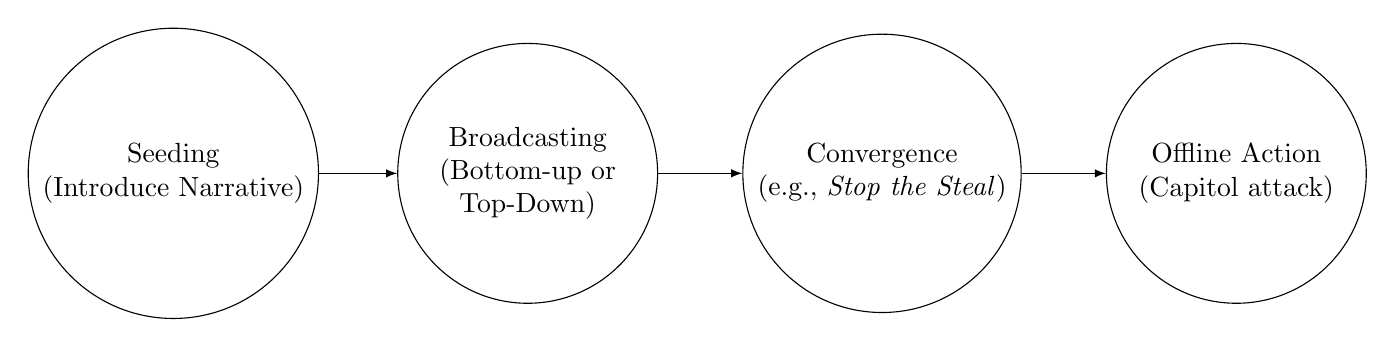
\begin{tikzpicture}[node distance=4.5cm, auto, >=latex]
      % Nodes (fixed size circles)
      \node[circle, draw, align=center, minimum size=3.3cm] (seed) {Seeding\\ (Introduce Narrative)};
      \node[circle, draw, align=center, right of=seed, minimum size=3.3cm] (amp) {Broadcasting\\(Bottom-up or \\ Top-Down)};
      \node[circle, draw, align=center, right of=amp, minimum size=3.3cm] (conv) {Convergence\\(e.g., \textit{Stop the Steal})};
      \node[circle, draw, align=center, right of=conv, minimum size=3.3cm] (act) {Offline Action\\(Capitol attack)};
      
      % Arrows
      \draw[->] (seed) -- (amp);
      \draw[->] (amp) -- (conv);
      \draw[->] (conv) -- (act);
    \end{tikzpicture}
    \caption{Stages of an \ac{io} leading to offline mobilization}
    \label{fig:IO-stages}
\end{figure}

\subsection{Social Network Graph Representation}

\subsubsection{Similarity Graphs} 

A \textit{similarity network} is a user-user graph representation designed to capture coordinated behavior among users by linking them according to behavioral resemblance. In this network, users who act in similar ways in the online environment are connected. The similarity is usually measured through \textit{co-action}, as described in Section~4.1.1. Typically, the weight of an edge increases with the degree of resemblance between users. 

The construction of such networks can follow two main approaches. The first approach is to directly measures user resemblance from the social network data, for example through sentiment or textual similarity analysis of posted content. The second approach begins with a user-entitie bipartite graph that connects users to entities derived from behavioral traces or co-actions (e.g., hashtags, URLs, or tweets). The weight of the edge reflects the frequency or intensity of a user’s interaction with a given entity. Using node embedding each user is then represented as a vector of entity usage. A similarity score is calculated according to the similarity between the users vectors,often computed through \textit{cosine similarity}. The similarity network contains these users and edges between users are weighted according to the similarity score. \cite{luceri2024unmasking, uncovering2021networks}.

Examples of similarity networks include the \textit{\ac{cp}} and the \ac{rrn}. 
A \textit{CopyPasta Network} is a similarity graph that connects users who share highly similar textual content (excluding identical retweets). By capturing these near-duplicate “copypasta” tweets, the network exposes coordinated efforts aimed at amplifying messages and fabricating the perception of widespread agreement \cite{coordinated2024Capitol}. 
A \ac{rrn} is a similarity graph which captures coordination by linking a user who re-shares a tweet to the original poster when the retweet occurs within a short time window. Edges are weighted by the number of such rapid retweets, with low-weight links filtered out to reduce noise \cite{unveiling2020whiteHelmets, coordinated2024Capitol}.


\begin{figure}[ht]
    \centering
    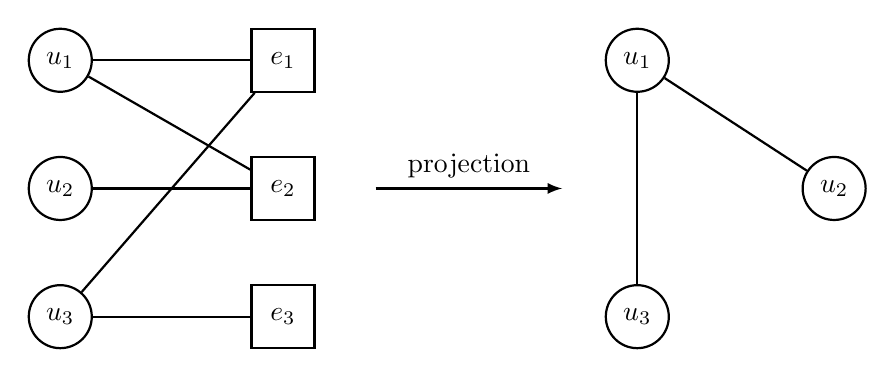
\begin{tikzpicture}[>=latex, thick, node distance=1.5cm]

        % User nodes
        \node[circle, draw, minimum size=0.8cm] (u1) {$u_1$};
        \node[circle, draw, below=0.8cm of u1, minimum size=0.8cm] (u2) {$u_2$};
        \node[circle, draw, below=0.8cm of u2, minimum size=0.8cm] (u3) {$u_3$};

        % Entity nodes
        \node[rectangle, draw, right=2cm of u1, minimum width=0.8cm, minimum height=0.8cm] (e1) {$e_1$};
        \node[rectangle, draw, right=2cm of u2, minimum width=0.8cm, minimum height=0.8cm] (e2) {$e_2$};
        \node[rectangle, draw, right=2cm of u3, minimum width=0.8cm, minimum height=0.8cm] (e3) {$e_3$};

        % Bipartite edges
        \draw (u1) -- (e1);
        \draw (u1) -- (e2);
        \draw (u2) -- (e2);
        \draw (u3) -- (e1);
        \draw (u3) -- (e3);

        % Arrow to similarity graph
        \node[right=0.5cm of e2] (arrowLabel) {};
        \draw[->, thick] (arrowLabel) -- ++(2.5,0) node[midway, above] {projection};


        % Similarity graph (users only)
        \node[circle, draw, right=6.5cm of u1, minimum size=0.8cm] (su1) {$u_1$};
        \node[circle, draw, right=9cm of u2, minimum size=0.8cm] (su2) {$u_2$};
        \node[circle, draw, right=6.5cm of u3, minimum size=0.8cm] (su3) {$u_3$};

        % Similarity edges
        \draw (su1) -- (su2);
        \draw (su1) -- (su3);

    \end{tikzpicture}
    \caption{Construction of a similarity network: users are first connected to entities in a bipartite graph, which is then projected into a user–user similarity graph.}
    \label{fig:similarity_graph}
\end{figure}

\paragraph{\Acl{fsn}} 
A \ac{fsn} integrates multiple behavioral traces into a single graph to capture a broader range of coordination signals. Instead of relying on a single similarity network (e.g., co-retweet or co-URL), the fused approach links two users if they are connected in any of the individual similarity networks. This fusion enhances robustness, since IO campaigns often employ diverse strategies that no single trace can fully capture. \cite{luceri2024unmasking,minici2025iohunter}.

\subsubsection{Information Diffusion Graphs}  
The process of information diffusion in social media can be captured through a \textit{diffusion graph}. The \textit{diffusion graph} are often a directed tree, also called \textit{spreading cascade}, where the root is the first adopter and branches indicate subsequent transmissions. In practice, multiple diffusion graphs may coexist, and different mergings of \textit{spreading cascades} can be considered. \textit{Diffusion graph} reflects both structural and temporal aspects. The structural aspects is manifested as the graph encodes who influenced whom. The temporal aspects is manifested as the diffusion graph describes the evolution of the adoption rate, i.e., the number of users who receive and propagate the information over time. Each node in the graph can be either inactive or activate, where activation denotes that a user has adopted a piece of information and attempts to spread it further. This graph-based view provides a foundation for reconstructing diffusion paths, quantifying cascade growth, and analyzing how influence and IOs propagates across the network.\cite{information2013diffusion}

\subsection{Graph Compression for Classification}

Graph reduction is fundamental for enhancing the efficiency and accuracy of graph-based classification models, including those applied to detecting \ac{io}. From a performance perspective, storage-efficient graph processing allows larger portions of data to fit into cache memory, reducing costly database accesses and minimizing the need for powerful hardware \cite{graphCompression2018survey}.  
From an accuracy perspective, its main benefit lies in filtering out irrelevant and noisy elements, enabling models to focus on meaningful signals. Thereby improving both robustness and reliability. This applies not only to random noise but also to adversarial attacks targeting the classification process \cite{backbone2022collectiveBehavior, graphClassification2023egc2}.

Social media platforms inherently generate large and complex network structures, often burdened with redundant or irrelevant interactions \cite{efficient2023eventDetection}. Such noise can obscure essential patterns, hindering accurate classification. By reducing graphs to emphasize salient features and relationships, models can more effectively extract discriminative structures associated with \ac{io} or \acp{cib}, thereby improving both predictive accuracy and interpretability \cite{backbone2022collectiveBehavior}.  

Graph compression techniques aim to simplify complex graphs while preserving their key structural properties. These methods rely on node and graph-level features from graph theory, such as degree and centrality, and may further integrate problem-specific characteristics from the relevant application domain \cite{graphCompression2018survey}.  
An example is \ac{ncp}, which prunes less significant nodes to refine graph structure \cite{NodeCentric2024Pruning}. A task-specific example is the \ac{kpg} framework, which generates enhanced key propagation graphs for rumor detection. This framework employs \ac{ens} framwork to identify critical nodes by assessing the contribution of their features and topological context to the classification performance \cite{RumorDetection2025GraphGenerator}.  




\subsection{IO Detection Methods}

At the core of coordination detection methods lies the assumption that genuine users operate independently, thus exhibiting limited
similarities in their online behaviors . Consequently, any unexpected convergence in behavior can hint at some kind of orchestration. \cite{uncovering2021networks, mannocci2024detection, unveiling2020whiteHelmets}

\subsubsection{Node-Local Methods}

While user-level methods are effective for identifying trolls through patterns of antisocial behavior, they are limited when it comes to detecting large-scale patterns such as IO. 
Such operations often rely on coordination across multiple accounts rather than the behavior of a single 
user. Therefore, user-level approaches can highlight individual malicious actors, but they do not capture the broader network structures that characterize coordinated campaigns. \cite{troll2020detection}

\paragraph{Post-based Methods} Post-based approaches rely on the analysis of the textual content produced by users. 
They apply natural language processing (NLP) techniques such as \textit{n-gram analysis}, 
\textit{readability metrics} (e.g., ARI, Flesch–Kincaid), and \textit{sentiment analysis} to 
detect patterns of hostility or provocation in text. More advanced directions include 
\textit{semantic models} such as \textit{sentic computing}, which capture the underlying meaning 
and emotional intent of the text. Metadata features like comment length, frequency of offensive 
terms, or posting time can also be considered as part of this category. \cite{TrollDetection2015sentiment}

\paragraph{User-based Methods} User-based approaches shift the focus from single posts to the broader activity of individuals across their participation in online discussion. These methods study features such 
as \textit{posting frequency}, \textit{temporal activity patterns}, and \textit{engagement with other users} through replies and interactions. They also consider \textit{community reactions}, including votes, reports, and flags, as well as \textit{moderator actions} like post deletions or bans. Furthermore, the \textit{distribution of topics} in which a user participates provides additional information about long-term conduct. Together, these signals help to characterize user behavior beyond isolated messages. \cite{trolls2014decluttering}

\subsubsection{Network-Based Methods}
\paragraph {\textit{Low-Weight Edge Filtering}} (unsupervised method) Edge filtering has long been one of the predominant techniques for detecting coordinated activity in social networks. The central assumption is that the similarity strength between users can reveal orchestrated behavior. In a similarity network, the weight of an edge encodes this similarity. By applying a similarity threshold, weaker ties are pruned, leaving behind clusters of users with unusually strong behavioral alignment. Users who lose all connections after filtering are generally not considered coordinated. \cite{uncovering2021networks, luceri2024unmasking, SocioLinguistic2024coordinated}

\paragraph{Node Pruning} (unsupervised method) Node pruning is a method that take similarity networks and removing accounts that are unlikely to play a central role in coordination. The idea is that coordinated actors often appear in central positions in the network, since they share strong similarities with many others. To capture this, centrality measures such as eigenvector centrality are applied, which evaluate not only how many connections a node has, but also how important its neighbors are. Accounts with very low centrality values are pruned, leaving a cleaner network that highlights the most influential and potentially coordinated actors. \cite{luceri2024unmasking, minici2025iohunter, mannocci2024detection}

\paragraph{Node Embedding and Classifier} (supervised methods) Node embedding methods, such as \textit{node2vec, DeepWalk, or Laplacian Eigenmaps,} map each node (user) in a social network to a low-dimensional vector space that captures structural properties of the graph. Once accounts are represented as feature vectors, a machine learning model serving as classifier (e.g., logistic regression, random forest) can be trained to distinguish IO accounts from organic users. \cite{Inductive2023graphLearning, mannocci2024detection}

\paragraph{\Ac{gnn}} (supervised method) \Acp{gnn} are a family of deep learning models designed to operate directly on graph-structured data. They work by iteratively aggregating and transforming information from a node’s neighbors, producing embeddings that capture both local features and global relational structure. These embeddings can then be used for a variety of tasks, with node classification being one of the most common task . A classifier layer, often a simple linear transformation with softmax, maps the embeddings to labels. \cite{GNN2022classification}

\paragraph{\Ac{gfm}} (supervised method) Recent developments in \acp{gfm} aim to pretraining large, general-purpose models on diverse graph data, enabling the model to handel a wide range of classification tasks. \acp{gfm} extend the foundation model paradigm to the graph domain, offering the potential for more robust cross-domain generalization as well as the simplicity of using off-the-shelf models. \cite{liu2025GFM, oneGraphModel2023classification}

\subsubsection{Hybrid Methods}

Hybrid approaches that combine textual and graph-based signals offer notable advantages in the detection of \acp{io}. Textual analysis alone captures semantic and narrative features, while graph-based analysis emphasizes structural and relational coordination. By integrating both approaches, hybrid methods exploit the complementarity of these modalities, enabling the detection \acp{io}. \cite{Inductive2023graphLearning, brugere2018network, minici2025iohunter, LLM2024IOdetecttion}

\begin{figure}[ht]
    \centering
    \makebox[\textwidth][c]{
        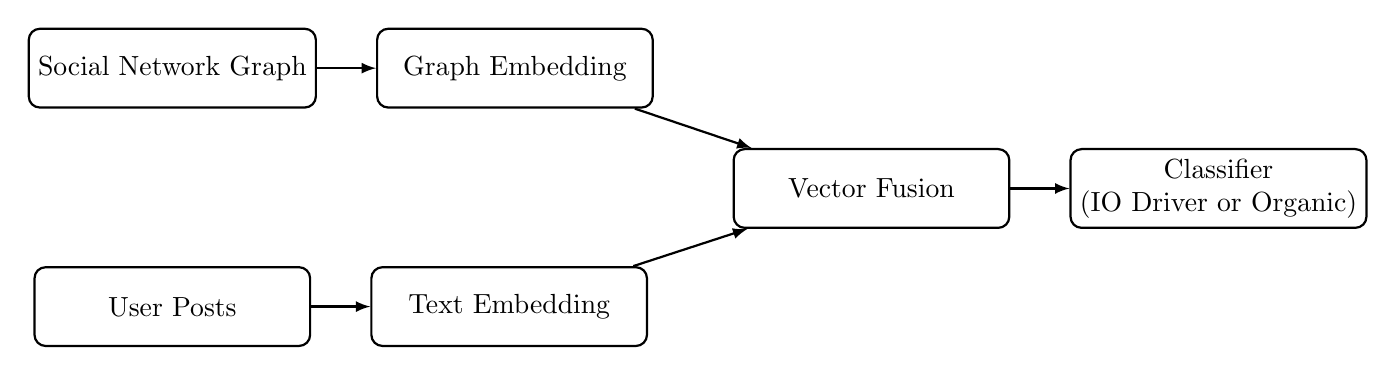
\begin{tikzpicture}[node distance=1cm, auto, >=latex, thick]

            % Input nodes
            \node[rectangle, draw, rounded corners, align=center, minimum width=3cm, minimum height=1cm] (graph) {Social Network Graph};
            \node[rectangle, draw, rounded corners, below=2cm of graph, align=center, minimum width=3.5cm, minimum height=1cm] (text) {User Posts};

            % Embeddings
            \node[rectangle, draw, rounded corners, right=0.75cm of graph, align=center, minimum width=3.5cm, minimum height=1cm] (graphEmb) {Graph Embedding};
            \node[rectangle, draw, rounded corners, right=0.75cm of text, align=center, minimum width=3.5cm, minimum height=1cm] (textEmb) {Text Embedding};

            % Fusion node (centered between embeddings)
            \node[rectangle, draw, rounded corners, below right=0.5cm and 1cm of graphEmb, align=center, minimum width=3.5cm, minimum height=1cm] (fusion) {Vector Fusion};

            % Classifier
            \node[rectangle, draw, rounded corners, right=0.75cm of fusion, align=center, minimum width=3.5cm, minimum height=1cm] (classifier) {Classifier \\ (IO Driver or Organic)};

            % Arrows
            \draw[->] (graph) -- (graphEmb);
            \draw[->] (text) -- (textEmb);
            \draw[->] (graphEmb) -- (fusion);
            \draw[->] (textEmb) -- (fusion);
            \draw[->] (fusion) -- (classifier);

        \end{tikzpicture}
    }
    \caption{General pipeline of hybrid methods for IO detection, showing left-to-right data flow from structural and textual inputs to classification.}
    \label{fig:hybrid pipeline}
\end{figure}



\paragraph{Case Study: IOHunter} \textit{IOHunter} is a detecting \acp{io} framework. It was developed as a \ac{gfm} that integrates multiple modalities within a unified architecture. The approach combines user's text, behavioral similarity networks, graph embeddings, cross-attention mechanisms and a \ac{gnn} classifier. First, fused similarity network are constructed from behavioral traces such as co-URL sharing, co-hashtag usage, and fast-retweet patterns. The similarity networks capture structural signals of the user interactions. The network is then processed by a \ac{gnn} encoder, producing node-level graph embeddings that represent the structural position of each user. In addition, textual content from user posts is embedded using the \texttt{SBERT} model, yielding vector representations that capture semantic properties of the text. The graph embeddings and textual embeddings are aligned through a cross-attention mechanism, which assigns relative importance to each modality and produces a fused representation. Finally, the fused vectors are passed through a \ac{gnn}-based classifier that performs user-level classification, distinguishing \acp{io} drivers from organic accounts \cite{minici2025iohunter}.

\subsection{Positioning of This Work Within the Research Field}
Prior research on information operations has largely concentrated on developing new detection algorithms or combining existing methods into complete detection frameworks. In contrast, this study does not aim to design a new classifier or construct an end-to-end pipeline. Instead, we addresses the fundamental problem of graph construction from social network data, with a particular focus on how different graph representations influence the performance of known IO detection approaches. We compare alternative graph representations designated to be inputs for graph-based or hybrid detection methods.

Unlike most prior studies, which treat the social network graph as a fixed input to detection algorithms, this work explicitly interrogates the construction of that graph itself. The analysis centers on how alternative graph representations, derived from heterogeneous social media data, shape both the accuracy and robustness of detection outcomes. By examining graph construction as an independent research problem, the study shifts attention to the fundamental representational step. 



\section{Methodology?}

\begin{figure}[h]
\centering
\begin{tikzpicture}[
  font=\small,
  node distance=10mm and 14mm,
  box/.style={
    rectangle,
    rounded corners=2mm,
    draw,
    thick,
    align=center,
    minimum width=30mm,
    minimum height=10mm
  },
  arrow/.style={-{Stealth[length=2.2mm]}, thick}
]

% -------- Top row --------
\node[box] (s1) {1) Cleaning, Translation,\\ NER};
\node[box, right=of s1] (s2) {2) Entity Reuse \\Identification};
\node[box, right=of s2] (s3) {3)  Narratives {\fontsize{8}{8}\selectfont(Sub-Topics)}\\Modeling};
\node[box, right=of s3] (s4) {4) Entities Scoring};

% -------- Bottom row --------
\node[box, below=14mm of s1] (s5) {5) Posts \& Authors\\Scoring};
\node[box, below=14mm of s2] (s6) {6) Key Authors Selection};
\node[box, below=14mm of s3] (s7) {7) Backbone Graph\\Building};
\node[box, below=14mm of s4] (s8) {8) \ac{io} Indicators\\ Calculation

};

% -------- Arrows (top row) --------
\draw[arrow] (s1) -- (s2);
\draw[arrow] (s2) -- (s3);
\draw[arrow] (s3) -- (s4);

% -------- Downward transition --------
% define the bend point
\coordinate (agg) at ($(s4.south)+(0,-6mm)$);

% draw arrow
\draw[arrow] (s4.south) -- (agg) -| (s5.north);

% place label exactly at center of horizontal segment
\node[
fill=black!60,
text=white,
rounded corners=4pt,
inner xsep=8pt,
inner ysep=3pt,
font=\small
]
at ($(agg)!0.5!(s5.north |- agg)$)
{Aggregation};


% -------- Arrows (bottom row) --------
\draw[arrow] (s5) -- (s6);
\draw[arrow] (s6) -- (s7);
\draw[arrow] (s7) -- (s8);

\end{tikzpicture}
\caption{From posts to backbone graph and \ac{io} indicators, workflow.}
\label{fig:workflow}
\end{figure}

\section{Results}

\section{Experiments}

\section{Conclusions}

\section{Acknowledgements}


\bibliographystyle{unsrt}
\bibliography{references}


\end{document}
